\documentclass[10pt,a4paper]{article}
\usepackage[usenames,dvipsnames]{xcolor}
\usepackage{tikz} % for drawing figures
\usepackage{amsmath} % for equations
\usepackage{url} % for URLs
\usepackage{graphicx}
\usepackage{multicol}
\usepackage{varwidth}
\usepackage{blindtext}
\usepackage{nicefrac}
\usepackage{enumerate}
\usepackage{booktabs}

\usepackage{linguex} % ** special include in directory: for doing handy example labeling and bracketing
\renewcommand{\firstrefdash}{} % used for linguex package not to put hyphens in example refs (1a instead of 1-a)
\usepackage{cogsci}
\usepackage{pslatex}
\usepackage{apacite}

\newcommand{\sem}[1]{\mbox{$[\![$#1$]\!]$}}
\newcommand{\den}[1]{\ensuremath{[\![#1]\!]}}
\newcommand{\lam}{$\lambda$}
\newcommand{\gcs}[1]{\textcolor{blue}{[gcs: #1]}} 
\newcommand{\mf}[1]{\textcolor{BrickRed}{[mf: #1]}} 
\newcommand{\tuple}[1]{\ensuremath{\langle #1 \rangle}} 

%%%%%%%%%%%%%%%%%%%%%%%%%%%%%%%%%%%%%%%%%%%%%%%%%%%%%%
%% for R_eproducible_LaTeX
%%%%%%%%%%%%%%%%%%%%%%%%%%%%%%%%%%%%%%%%%%%%%%%%%%%%%%

\usepackage{pgfplotstable}
\usepackage{csvsimple}
% \usepackage{siunitx}

% set the name of the folder in which the CSV files with 
% information from R is stored
\newcommand{\datafoldername}{R_data_4_TeX}

% the following code defines the convenience functions
% as described in the main text below

% rlgetvalue returns whatever is the in cell of the CSV file
% be it string or number; it does not format anything
\newcommand{\rlgetvalue}[4]{\csvreader[filter strcmp={\mykey}{#3},
             late after line = {{,}\ }, late after last line = {{}}]
            {\datafoldername/#1}{#2=\mykey,#4=\myvalue}{\myvalue}}

% rlgetvariable is a shortcut for a specific CSV file (myvars.csv) in which
% individual variables that do not belong to a larger chunk can be stored
\newcommand{\rlgetvariable}[1]{\csvreader[]{\datafoldername/myvars.csv}{#1=\myvar}{\myvar}\xspace}

% % rlnum format a decimal number
% \newcommand{\rlnum}[2]{\num[output-decimal-marker={.},
%                              exponent-product = \cdot,
%                              round-mode=places,
%                              round-precision=#2,
%                              group-digits=false]{#1}}

% \newcommand{\rlnumsci}[2]{\num[output-decimal-marker={.},
%                           scientific-notation = true,
%                              exponent-product = \cdot,
%                              round-mode=places,
%                              round-precision=#2,
%                              group-digits=false]{#1}}

% \newcommand{\rlgetnum}[5]{\csvreader[filter strcmp={\mykey}{#3},
%              late after line = {{,}\ }, late after last line = {{}}]
%             {\datafoldername/#1}{#2=\mykey,#4=\myvalue}{\rlnum{\myvalue}{#5}}}

% \newcommand{\rlgetnumsci}[5]{\csvreader[filter strcmp={\mykey}{#3},
%              late after line = {{,}\ }, late after last line = {{}}]
%             {\datafoldername/#1}{#2=\mykey,#4=\myvalue}{\rlnumsci{\myvalue}{#5}}}

%%%%%%%%%%%%%%%%%%%%%%%%%%%%%%%%%%%%%%%%%%%%%%%%%%%%%%
%%%%%%%%%%%%%%%%%%%%%%%%%%%%%%%%%%%%%%%%%%%%%%%%%%%%%%

\title{Subjectivity-based adjective ordering maximizes communicative success}
%\author{\large \textbf{Michael Franke$^1$, Gregory Scontras$^2$, Mihael Simoni\v{c}$^3$}\\
%  $^1$ Institute for Cognitive Science, University of Osnabrueck (michael.franke@uos.de)\\
%  $^2$ Department of Language Science, University of California, Irvine (g.scontras@uci.edu)\\
%  $^3$ Humanoid and Cognitive Robotics Lab, Jo\v{z}ef Stefan Institute,
%  Ljubljana (mihael.simonic@ijs.si)}


\begin{document}
\maketitle

\begin{abstract}
  
Adjective ordering preferences (e.g., \emph{big brown bag} vs.~\emph{brown big bag}) are robustly attested in English and many unrelated languages \cite{dixon1982}. \citeA{scontrasetal2017adjectives} showed that adjective subjectivity is a robust predictor of ordering preferences in English: less subjective adjectives are preferred closer to the modified noun. In a follow-up to this empirical finding, \citeA{simonic2018} and \citeauthor{scontrasetalSPadjectives} (to appear) claim that pressures from successful reference resolution and the hierarchical structure of modification explain subjectivity-based ordering preferences. We provide further support for this claim using large-scale simulations of reference scenarios, together with an empirically-motivated adjective semantics. In the vast majority of cases, subjectivity-based adjective orderings yield a higher probability of successful reference resolution.

\textbf{Keywords:} 
adjective ordering, subjectivity, reference resolution, hierarchical modification

\end{abstract}

\section{Introduction}

When speakers use two or more adjectives to modify a noun, they exhibit robust preferences in the relative order of the adjectives (e.g., \emph{big brown bag} vs.~\emph{brown big bag}). Using a series of behavioral and corpus experiments, \citeA{scontrasetal2017adjectives} demonstrated that adjective order in multi-adjective strings is reliably predicted by the subjectivity of the adjectives involved: less subjective adjectives are preferred closer to the modified noun, and the strength of the preference is modulated by the subjectivity differential between the adjectives. Thus, speakers strongly prefer \emph{big brown bag} over \emph{brown big bag}, as \emph{brown} is much less subjective than \emph{big}.

The question that immediately arises is why subjectivity should play the role it does in adjective ordering preferences. The current work follows \citeA{simonic2018} and \citeauthor{scontrasetalSPadjectives} (to appear) in advancing the claim that pressures from successful reference resolution deliver subjectivity-based ordering preferences. In certain cases of restrictive
modification which proceed incrementally based on syntax-driven meaning composition, adjectives that compose with the nominal later will classify a smaller set of potential referents (e.g., the set of bags vs. the set of brown boxs). We demonstrate that, in order to avoid alignment errors where a listener might mis-characterize the intended referent, it is, when averaging over many contexts of use, a better strategy to introduce the more error-prone (i.e., more subjective) adjectives later in the hierarchical meaning composition; the structure linearizes such that subjectivity decreases the closer you get to the modified noun. We build on the work that precedes ours by making minimal assumptions about online processing (cf.~\citeauthor{scontrasetalSPadjectives}, to appear) and by assuming a more principled implementation of adjective subjectivity within an empirically-motivated semantics (cf.~\citeNP{simonic2018}).

The paper is structured as follows. First, we review the empirical generalization concerning subjectivity-based preferences, together with the proposals offered to account for this generalization. Then, we consider empirical work on adjective semantics, which serves as inspiration for our own proposal. We demonstrate, using Monte Carlo simulation, how a minimal set of independently-motivated assumptions leads to a ready explanation for subjectivity-based ordering preferences: ordering adjectives with respect to decreasing subjectivity has a higher probability of successful reference resolution, when averaging across many contexts of use. 

\section{Background}

Given the robustness of adjective ordering preferences within and across languages, there has been no shortage of proposals meant to account for the regularities in adjective ordering. Some have offered grammatical proposals that attend to semantic composition or articulated syntactic hierarchies (e.g., \citeNP{cinque1994,scott2002,mcnallyboleda2004,truswell2009}). Others have advanced more psychological proposals built around notions like inherentness or accessibility (e.g, \citeNP{whorf1945,ziff1960,martin1969}). Recently, \citeA{scontrasetal2017adjectives} synthesized several proposals that preceded them and advanced the hypothesis that adjective subjectivity predicts ordering preferences (see also \citeNP{quirketal1985,hetzron1978,dixon1982,tucker1998,hill2012}). 

In order to test the subjectivity hypothesis, \citeA{scontrasetal2017adjectives}~first had to determine what the ordering preferences were. They established a behavioral measure of the preferences whereby experimental participants indicated the preferred ordering of multi-adjective strings that differed only in the relative order of the adjectives involved (e.g., \emph{the big brown bag} vs. \emph{the brown big bag}). \citeA{scontrasetal2017adjectives}~then validated their behavioral measure by comparing it with naturalistic productions from corpora. They found a high correlation between the behavioral and corpus measures ($r^{2}=.83, 95\%$ CI $[.63, .90]$), suggesting that the behavioral measure was successful in capturing the preferences speakers use when forming multi-adjective strings.

Next, \citeA{scontrasetal2017adjectives}~measured adjective subjectivity. They started by simply asking participants how ``subjective'' a given adjective was (e.g., ``How subjective is \emph{brown}?''). Wary of how naive participants might interpret the word ``subjective,'' the authors validated their subjectivity measure by comparing it with faultless disagreement scores \cite{kolbel2004,barker2013,kennedy2013,macfarlane2014}. In a faultless disagreement task, participants observe a disagreement between two speakers about whether an adjective applies to some object (e.g., whether or not a table is brown). The task is to decide whether the two speakers can both be right while disagreeing, or whether one of them must be wrong; to the extent that both speakers can be right, the adjective admits that degree of faultless disagreement. \citeA{scontrasetal2017adjectives}~found an extremely high correlation between the raw ``subjectivity'' scores and the faultless disagreement measure ($r^{2}=.91, 95\%$ CI $[.86, .94]$), suggesting that they had a reliable measure of adjective subjectivity.

Comparing the ordering preferences with adjective subjectivity, \citeA{scontrasetal2017adjectives}~found that subjectivity accounts for 85\% of the variance in the ordering preferences ($r^{2}=.85, 95\%$ CI $[.75, .90]$) for 26 different adjectives from seven semantic classes. The authors then looked at every multi-adjective string in the Switchboard corpus of English, finding that subjectivity accounts for 61\% of the variance in ordering preferences ($r^{2}=.61, 95\%$ CI $[.47, .71]$) for 74 unique adjectives from 13 semantic classes. In other words, the authors found strong support for their hypothesis that subjectivity predicts adjective ordering preferences. The question that immediately presents itself, however, is why subjectivity should matter in adjective ordering. \citeA{scontrasetal2017adjectives}~gesture toward an answer to this question---less subjective adjectives are more useful for establishing reference, and speakers consolidate the more useful, less subjective content around the modified noun---but their suggestion is purely speculative.

Using a model of probabilistic utterance choice (e.g., \emph{big brown bag} vs.~\emph{brown big bag}), \citeA{simonic2018} systematically explored the idea that subjectivity-based ordering preferences arise under pressure from successful reference resolution. The utterance choice model was formulated within the Rational Speech Act modeling framework \cite<e.g.,>{FrankeJager2015:Probabilistic-p,goodmanfrank2016}.\footnote{See \citeA{hahnetal2018} for a different approach to modeling adjective ordering within the Rational Speech Act framework. Their model defines speaker utility not in terms of referential success, but rather in terms of communicating subjective opinions about objects.} To model adjective subjectivity, the speaker assumes that the listener might have a different lexical meaning for each adjective. If $L_{adj}^{S,C}$ is the speaker's lexical entry for adjective $adj$ in context $C$, the speaker believes that the probability that the listener has a lexical entry $L_{adj}^{L,C}$ is:
\begin{align}
  \label{eq:SimonicErrors}
  P(L_{adj}^{L,C} \mid L_{adj}^{S,C}) \propto
  \begin{cases}
    1 & if L_{adj}^{S,C} = L_{adj}^{L,C} \\
    \epsilon_{adj} & \text{otherwise}
  \end{cases}
\end{align}
The more subjective the adjective, the higher the error probability $\epsilon_{adj}$. With these beliefs about lexical divergence, \citeauthor{simonic2018} shows that the subjectivity-based ordering \emph{big brown bag} is a more rational choice for the speaker than \emph{brown big bag} in a wide range \gcs{can we be more specific about how wide this range is (in line with the 100K / 93\% number in the summary of Scontras et al.)?} of randomly-generated contexts.

\citeauthor{scontrasetalSPadjectives}~(to appear) pursue a similar explanation for subjectivity-based ordering preferences. They treat adjective subjectivity as potential noise in the semantics of an adjective, similar to \citeauthor{simonic2018}, but they assume that, based on a ground-truth of objective adjective meaning, each agent (speaker or hearer) will incorrectly classify each potential referent in the current context $C$ with an error rate $\epsilon_{adj}$, which, again, indexes adjective subjectivity:
\begin{align}
  \label{eq:ScotrasError}
  \sem{ADJ}^C  = \lambda x \in C. & \textrm{ if } \texttt{ADJ}(x) \textrm{ then } 
  \texttt{flip}(1- \epsilon_{adj}),\\
  &  \textrm{ else } \texttt{flip}(\epsilon_{adj}) \nonumber
\end{align}
This move allows \citeauthor{scontrasetalSPadjectives} to treat deviations from the ground truth as gradient: greater deviation is increasingly less likely. \citeauthor{scontrasetalSPadjectives} further assume that each object classification requires some processing cost. As a result, the error probability $\epsilon_{adj}$ is assumed to increase with the size of context $C$. Based on these assumptions, \citeauthor{scontrasetalSPadjectives} demonstrate how subjectivity-based ordering preferences can maximize the probability of correctly classifying the intended referent. The authors explored 103,740 cases of multi-adjective modification and found that subjectivity-based ordering behaved as expected in 93\% of those cases.

In sum, both \citeA{simonic2018} and \citeauthor{scontrasetalSPadjectives}~(to appear) demonstrate how subjectivity-based adjective ordering serves successful referential communication. However, both accounts involve non-trivial and potentially controversial assumptions. \citeauthor{simonic2018}'s anything-goes assumption in \eqref{eq:SimonicErrors} concerning the speaker's beliefs about the listener's lexicon are not very intuitive: why, for instance, would the speaker believe that a small deviation from his own lexicon is equally likely as a massive deviation? \citeA{scontrasetalSPadjectives} likewise merely stipulate that error of classification $\epsilon_{adj}$ in \eqref{eq:ScotrasError} is a function of context size $C$. It would be much more desirable to derive divergences between the speaker's and listener's semantic classifications from more fundamental assumptions, first and foremost by a more explicit view of what the underlying semantics of adjectives is. Consequently, our aim here is to build on these previous accounts by showing how subjectivity-based ordering serves successful referential communication. However, rather than making what are now rather stipulative assumptions about the misalignment of semantic representations, we will show how these misalignments can arise from a generally plausible context-dependent semantics. It is to one such semantics that we turn next.


\section{Semantic assumptions}

%a subsective semantics where the meaning of the adjective depends on the meaning of the noun it modifies
%focus on how speakers identify things in the world as tall, short, big, or small.
%things may count as tall if they are taller than average, or taller than most things in a class (Barner & Snedeker, 2008).
%compare the performance of a number of possible models of tall to the tallness judgments of people
%using Bayesian methods to probabilistically cluster items
%compute a threshold statistic from the heights of the objects in the context, and make tallness judgements by comparing to this threshold
%normally-distrubuted noise on the threshold
%Relative height by range (RH-R): any item within the top k% of the range of heights is tall. If we write Mx = max x?C h(x) and Mn = min x?C h(x), then: T(C) = Mx?k (Mx?Mn).
%clustering model: an item is tall if it is in the same cluster as the tallest item; The shortest item is required to be in a separate category from the tallest item
%expt 1: Adult subjects judged which items were tall in a wide variety of distributions of items; all of the models that depend on the height of objects in a given distribution (RH-R, RH-SD, and CLUS) performed well overall
%the best RH-R threshold is k = 27% for Experiment 2 (with a noise parameter of ? = 0.01) and k = 29% overall

In their study of adjective meaning, \citeA{schmidtetal2009} began with the observation that gradable adjectives mean different things depending on the nouns they modify: what counts as big for a mouse diverges drastically from what counts as big for an elephant. The question, then, is what serves as the core meaning of a gradable adjective, such that speakers can determine its extension in context? 
 
To answer this question, \citeauthor{schmidtetal2009} collected human judgments about what counts as ``tall'' for different sets of objects. They then compared these judgments with the predictions from a number of semantic models that use various strategies to determine tallness in context. The strategies considered fell into one of two classes. The first class computed the tallness threshold directly, using various parametric and non-parametric procedures to compute a height cutoff above which objects count as tall. The second class inferred the tallness threshold on the basis of category membership, first performing a clustering analysis on the set of objects and then identifying as tall those objects that belonged to the cluster with the tallest object.

Two models outperformed the rest. The simplest was a threshold-computing model that sets the threshold on the basis of relative height by range: any object that fell within the top $k\%$ of the range of heights in context $C$ counts as tall in $C$. Formally, the set $\den{\text{tall}}^C$ of objects in $C$ that count as tall in $C$ is (where $\texttt{tall}(o)$ is the tallness of object $o$, \texttt{max} is the tallness of the tallest object in $C$, and \texttt{min} that of the smallest):
\begin{align}
  \label{eq:Semantics}
  \den{\text{tall}}^C  = & \ \{ o \in C \mid \texttt{tall}(o) \ge \texttt{max} - \theta \cdot (\texttt{max} - \texttt{min}) \} \,, \\
  & \text{ where $\theta = \nicefrac{k}{100}$.} \nonumber
\end{align}
So, if the maximum object height is 10 on the relevant scale and the minimum height is 2, a $k$ of 50\% would set the tallness threshold at 6; that is, an object with a height greater than 6 would count as tall in that context. Notably, the more complex clustering model performed no better than this threshold model when it came to predicting human judgments. We will therefore use this simple but empirically-motivated threshold semantics in the reasoning that follows, treating the threshold $\theta$ as a free model variable.

Following \citeA{simonic2018} and \citeA{scontrasetalSPadjectives}, we further assume that iterated adjectival modification triggers \emph{sequentially intersective context updates}. Later adjectives (syntactically farther from the modified noun) are interpreted relative to contexts that have already been restricted by previous adjectives. For example, the denotation of the phrase ``[adj\textsubscript{i} [adj\textsubscript{j} $N$]]'' given a shared context $C$ of potential referents is:
\begin{align}
  \label{eq:SequentialInterpretation}
  \den{\text{[adj\textsubscript{i} [adj\textsubscript{j} $N$]]}}^{C} & = \den{\text{adj}_i}^{\den{\text{adj}_j}^{C\cap \den{N}}} 
\end{align} 
In words, a string like ``big brown bag'' characterizes the set of all bags in context $C$ that count as brown (in the set of bags in $C$) and that count as big (in the set of bags that count as brown in the set of bags in $C$). Each adjective is therefore interpreted relative to its local context of incremental compositional semantic interpretation, so to speak. The effect is that adjectives closer to the noun will operate over a larger context (i.e., one that is less restricted); paired with a context-dependent semantics as in \eqref{eq:Semantics}, it is conceivable that the ordering of adjectives matters for referential success.


\section{Motivating example}

For the discussion that follows, we use ``brown'' and ``big'' as mnemonic labels for any two adjectives that are, respectively, less and more subjective. Our goal is to demonstrate why an utterance of ``big brown $X$''---that is, a multi-adjective string ordered with respect to decreasing subjectivity---is communicatively more efficient on average than an utterance of ``brown big $X$''---an utterance not ordered with respect to decreasing subjectivity. An utterance's average communicative success is spelled out here as the \emph{expected utility} in a situation where the speaker wants to refer to an object; this value is specified, consequently, as the average probability of getting the listener to choose the intended referent on the basis of that utterance.

\begin{figure}[t]
  \centering
 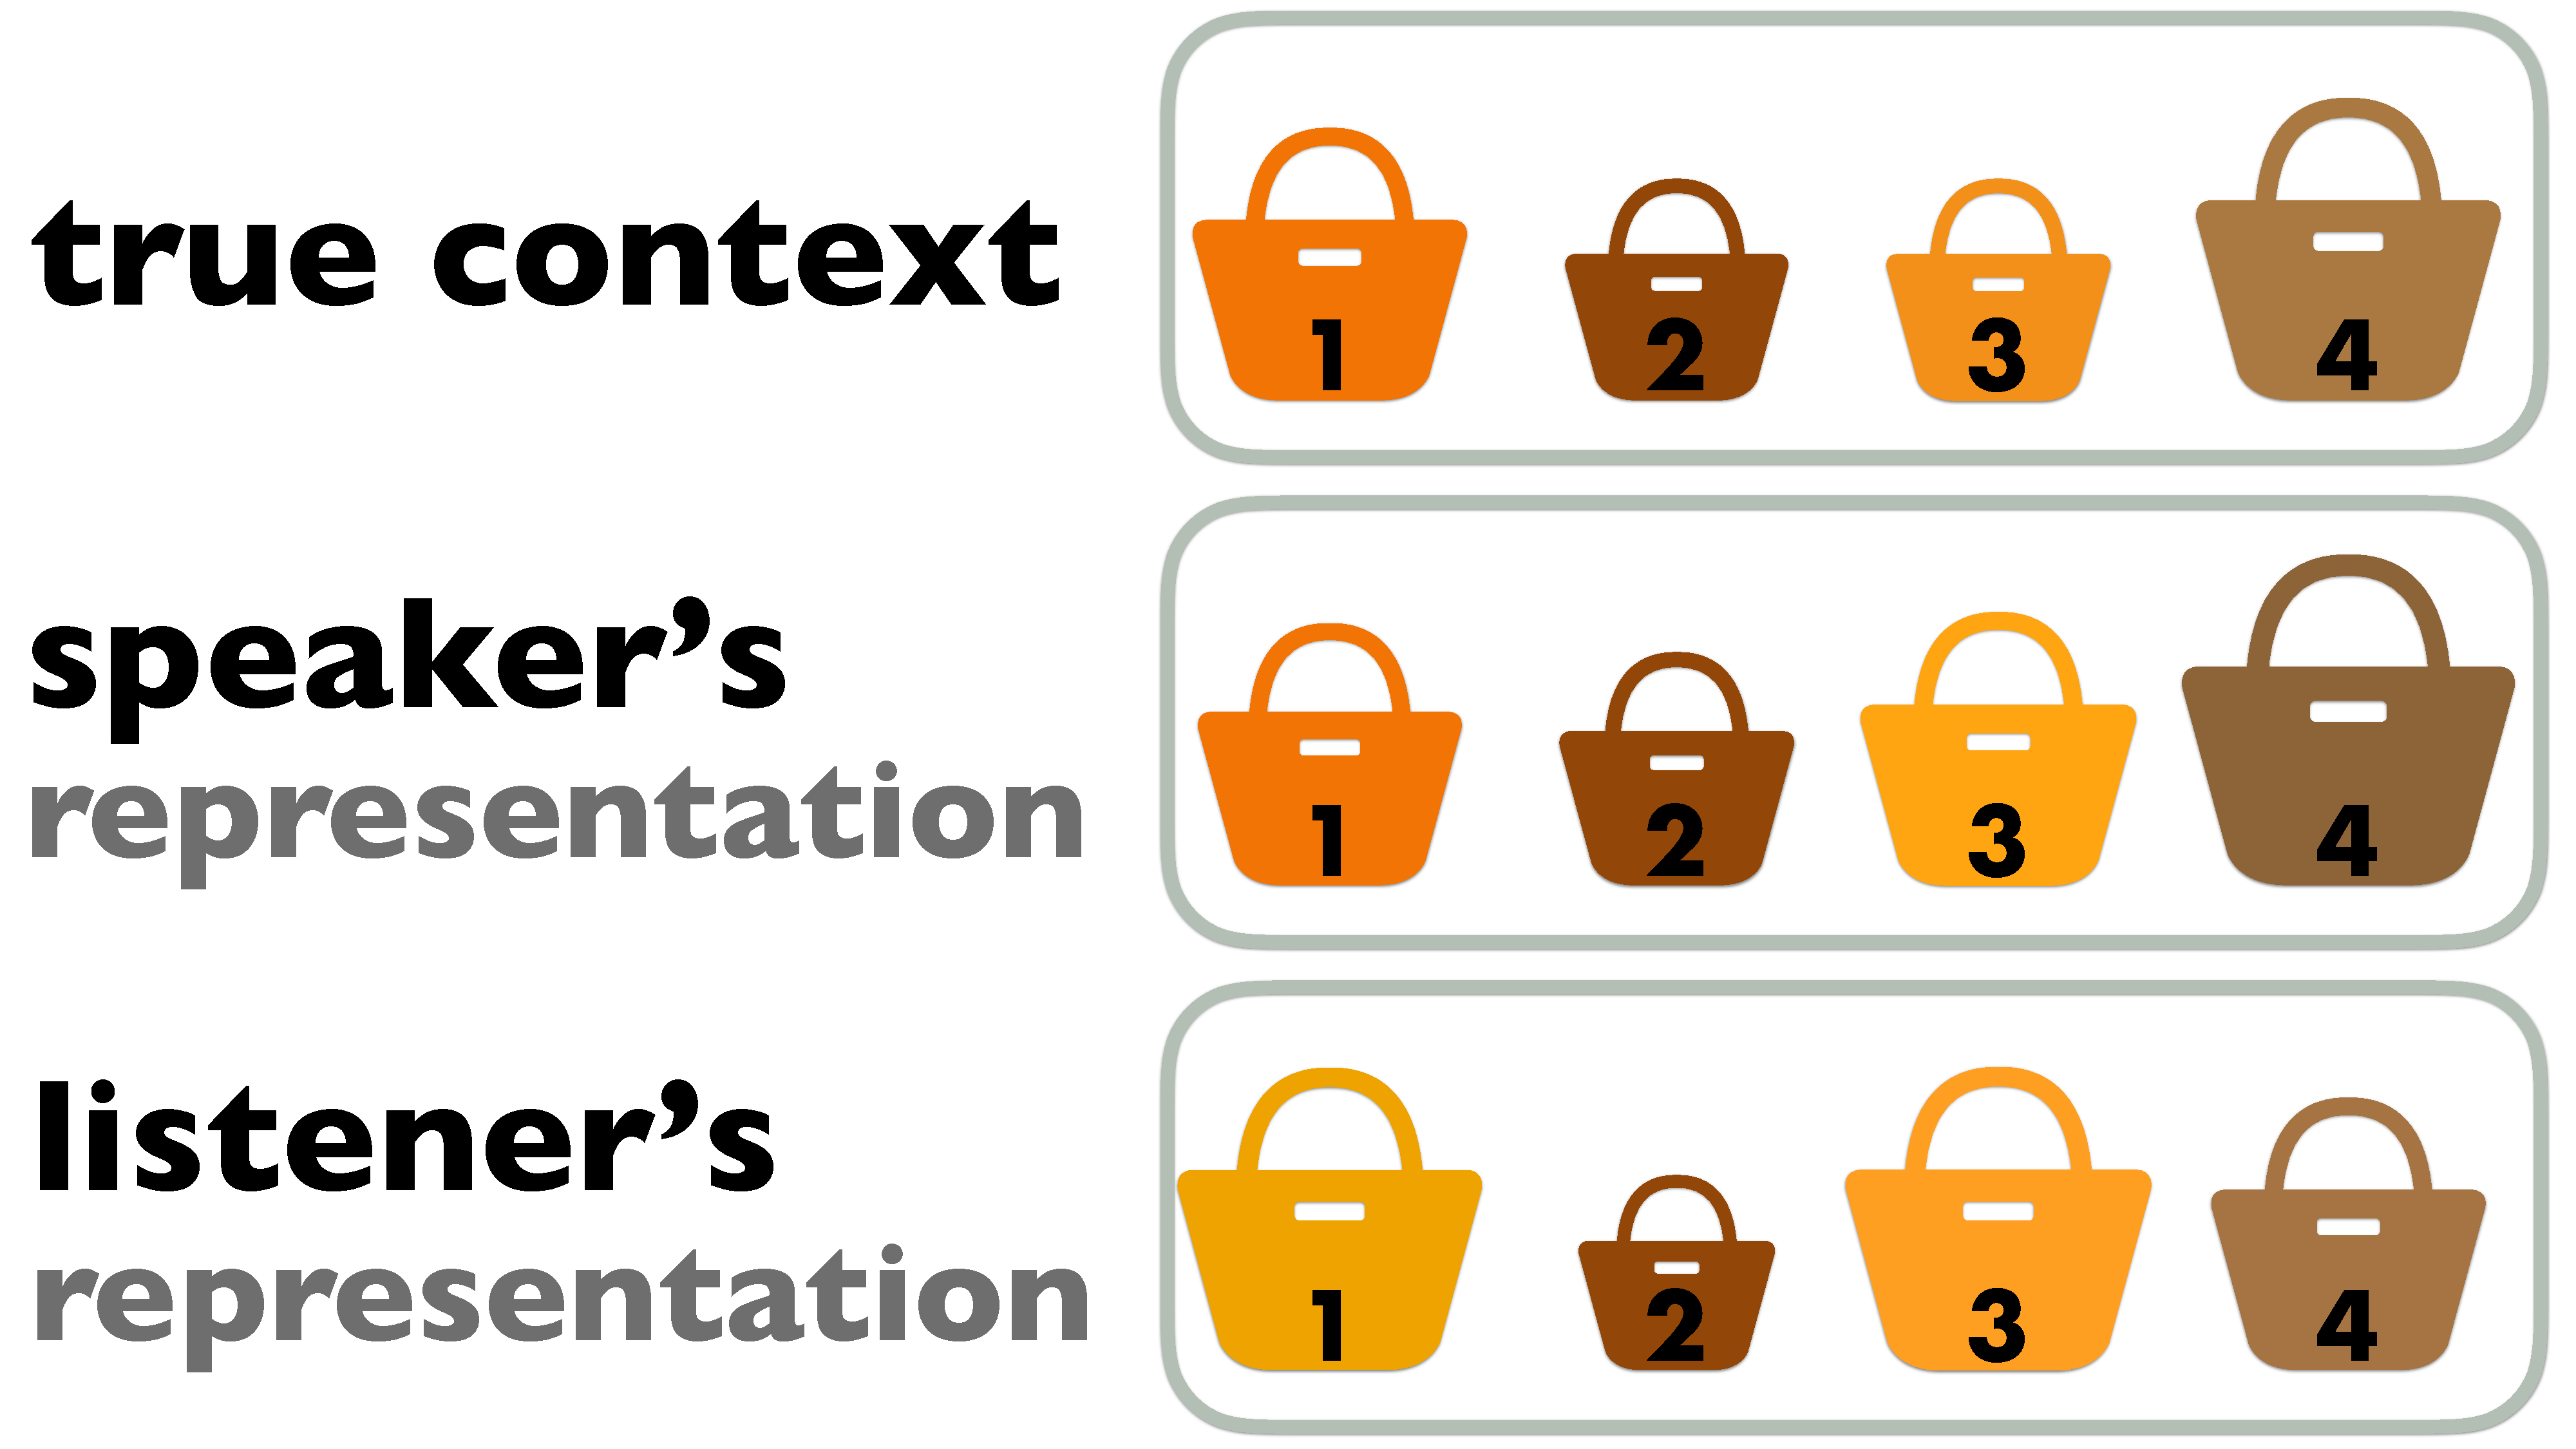
\includegraphics[width=.95\linewidth]{model_picture.pdf} 
 \vspace{-5pt}
  \caption{Illustration of subjective agent representations.}
  \label{fig:ModelIllustration}
\end{figure}

To get this reasoning off the ground, we first need to make some assumptions about the effects of adjective subjectivity on our mental representations---representations that will be relevant to referential communication. Figure~\ref{fig:ModelIllustration} gives a concrete example to illustrate the main idea. Suppose that the speaker and listener share access to a context of four bags that differ only with respect to color and size. Depending on their different perceptual angles, different background knowledge, or differences in previous experiences, the speaker and listener might represent the context differently: their impressions of object size and object color could deviate from the ground truth. 

Here is where subjectivity comes in: more subjective properties are more likely to lead to deviation between the ground truth (i.e., the true context) and an agent's representation of the property. Crucially, by deviating from the ground truth, these more subjective properties are also more likely to lead to deviations between two agent representations (e.g., between the speaker's and listener's representations in Figure \ref{fig:ModelIllustration}); these deviations \emph{and our awareness of their potential} are what lead to perceived subjectivity as measured by a faultless disagreement task. Language users are aware that their representations might deviate from each other's, and the potential for deviation is different for different properties. We illustrate this tendency in Figure \ref{fig:ModelIllustration}, where the agent representations of size deviate more from the ground truth than their representations of color.

We now ask: if the speaker wants to describe a bag that is both big and brown according to her subjective representation of the context, would it be better, on average, to describe it as ``big brown bag'' or ``brown big bag'', knowing that the listener would interpret either phrase from his own subjective perspective? Concretely, suppose the speaker wants to refer to bag 4 in Figure \ref{fig:ModelIllustration}, which is both brown and big from her subjective point of view. If the listener hears ``big brown bag'', he tries to find the speaker-intended referent by incrementally restricting the set of possible referents according to the interpretation rule in \eqref{eq:SequentialInterpretation}, applying the context-dependent semantics in \eqref{eq:Semantics} to his own subjective representation of the objects in question. For the example from Figure~\ref{fig:ModelIllustration} and assuming that $\theta = 0.5$ in \eqref{eq:Semantics}, the phrase ``brown bag'' would make the listener consider only bags 2 and 4. Of these, only bag 4 is in the top 50\% along the range of size in this context set. So, the interpretation of ``big brown bag'' is successful; the listener recovers the speaker-intended referent uniquely. In contrast, for the expression ``brown big bag'', the listener first looks at the bags that count as big, which rules out only bag 2, since it is the only bag whose size is in the lower 50\% of the range of sizes. Among the remaining bags (1, 3 and 4), bag 3 is clearly not brown. For the sake of this informal example, assume that the listener therefore considers both bags 1 and 4 as possible referents when hearing ``brown big bag''. The chance of referential success (i.e., choosing bag 4)---neglecting salience or other factors---would be $\nicefrac{1}{2}$, lower than the certain communicative success when interpreting ``big brown bag''.


\section{Computing average communicative success}

We use a Monte Carlo simulation to estimate the difference in expected referential success between phrases ``big brown bag'' and ``brown big bag''; we calculate this value by averaging over many different contexts with different numbers of objects and varying degrees of subjectivity for the properties involved. In this way, we are not assuming that agents themselves reason actively about the stochastic misalignment of semantic judgements, or that they choose expressions that are optimal with respect to these calculations. We merely compute the average communicative success of, say, a fictitious community of agents who would use ``big brown bag'' (i.e., subjectivity-based ordering) and compare their success to that of a different community that uses ``brown big bag'' instead. A single run of the Monte Carlo simulation proceeds as follows:

\begin{enumerate}
\setlength{\itemsep}{0pt}

\item We first sample a number $n$ of bags in the current context uniformly at
  random from 4 to 20.

\item For each object $o$, we sample the degree to which $o$ is brown and the
  degree to which it is big. These samples are obtained from independent draws
  from a standard normal distribution. This sampling yields a representation of
  the \emph{actual context} $C$ as an $n \times 2$ matrix of feature values for
  the $n$ objects. The probability of sampling context $C$ for fixed $n$ is
  \begin{align*}
    P(C \mid n) = \prod_{i=1}^n \prod_{j=1}^2 \mathcal{N}(C_{ij} \mid \mu = 0, \sigma = 1)\,.
  \end{align*}

\item Agent $X$'s (speaker's or listener's) subjective representation $C^X$ of
  $C$ is derived from $C$ by assuming normally distributed noise around the
  property degrees in $C$, with a fixed standard deviation for each adjective.
  The probability of obtaining a subjective representation $C^X$ from the actual
  context $C$ is
  \begin{align*}
    P(C^X \mid C) = \prod_{i=1}^n \prod_{j=1}^2 \mathcal{N}(C_{ij}^X \mid \mu = C_{ij}, \sigma = \sigma_j)\,.
  \end{align*}
  The standard deviations $\sigma_{1,2}$ are obtained by sampling two numbers
  uniformly from the interval $[0;0.5]$ and assigning the higher number to the
  more subjective adjective (``tall'') and the lower number to the less subjective
  adjective (``brown'').

\item A \emph{semantic threshold} $\theta \sim \mathcal{U}(0,1)$ is sampled
  uniformly at random from the unit interval. We apply the context-dependent
  threshold semantics in \eqref{eq:Semantics} from \citeA{schmidtetal2009} with
  the incrementally intersective context update in
  \eqref{eq:SequentialInterpretation}, using each agent's subjective context
  representation, to yield each agent's subjective interpretation of each
  referential phrase.\footnote{In this way, the actual context $C$ plays no role
    in the assignment of subjective truth conditions; $C$ is just a means of
    efficiently sampling subjective context representations that are more or
    less aligned with each other. \gcs{I'm not sure I understand what you're trying to say here.}}
  % The denotation $\sem{adj\textsubscript{j}}^{C}$ of adjective $j \in \{1,2\}$
  % relative to some context $C$ (actual or subjective; possibly further
  % restricted by previous adjectival modification) is the set of all objects
  % $i$ such that $C_{ij} > \max_{i'}C_{i'j} - \theta \cdot (\max_{i'}C_{i'j} -
  % \min_{i'}C_{i'j})$.
 
\item We then sample the \emph{speaker-intended referent object} $i^*$ randomly
  from the set $\den{\text{adj}_1}^{C^S} \cap \den{\text{adj}_2}^{C^S}$ (i.e.,
  an object that is both brown and big from the point of view of the speaker).
  If there is no such object, the run is discarded.
  
\item If the listener's interpretation of the phrase ``[adj\textsubscript{i}
  [adj\textsubscript{j}]]'' from his subjective point of view is $I =
  \den{\text{[adj\textsubscript{i} [adj\textsubscript{j}]]}}^{C^L}$, the
  probability of recovering the intended referent is $|I|^{-1}$ if $i^* \in I$
  and 0 otherwise. We record the probability of recovery for both adjective
  orders and evaluate their distribution over all samples obtained in this way.

\end{enumerate}



\section{Results}

Based on $10^5$ Monte Carlo samples from the process outlined above, we estimate the expected probability of recovering the speaker's intended referent with the subjectivity-based ordering ``big brown bag'' as \rlgetvariable{EU_big_brown}, compared to \rlgetvariable{EU_brown_big} for the reverse ordering ``brown big bag''. The obtained samples of expected utilities for each ordering appear to indeed be different  (paired $t$-test, $t \approx \rlgetvariable{Tstatistic}$, $p < 10e^{80}$). The direction of this difference lends credence to the general idea that, on average,  ordering adjectives by subjectivity does affect average referential success, and that using the less subjective adjective early in sequential interpretation is communicatively beneficial. In other words, ordering adjectives with respect to decreasing subjectivity increases the probability of communicative success.

To understand these results better, Figure~\ref{fig:Showcase_examples} shows results from Monte Carlo simulations for a small selection of the parameter values we investigated. We limit our focus to values for standard deviations $\sigma_{\text{brown}} \in \{0.1, 0.2\}$ and $\sigma_{\text{big}} \in \{0.25, 0.3\}$ for the subjective agent representations; we consider semantic threshold values $\theta \in \{ 0.2, 0.4, 0.6, 0.8 \}$. For each combination of these values, we ran 10,000 simulations following the procedure outlined above. The vertical axis in Figure~\ref{fig:Showcase_examples} plots two measures. Upward from the 0-mark is the difference in mean communicative success between ``big brown bag'' and ``brown big bag''. We see that all mean values are positive, which signals that for all parameter constellations picked out here, the phrase ``big brown bag'' was indeed estimated to be communicatively more successful in each case. Below the 0-mark in Figure~\ref{fig:Showcase_examples}, we see the percentage of simulation runs in which the reverse ordering ``brown big bag'' had a higher expected utility. This shows that the communicative advantage of one adjective ordering over another is not absolute: there are exceptions. However, when averaging over all cases, there is nonetheless a clear communicative benefit of ``big brown bag'' over ``brown big bag''.

\begin{figure}
  \centering
  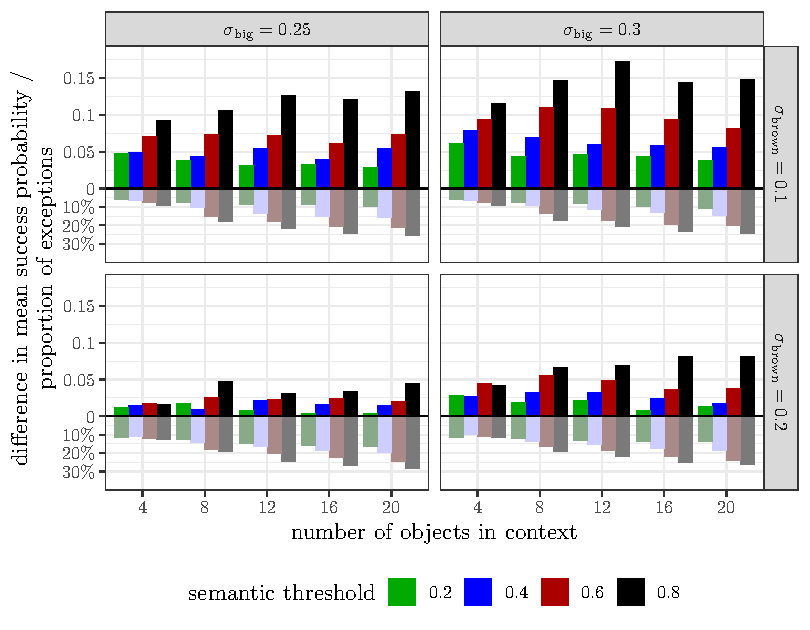
\includegraphics[width = \linewidth]{plots/tikz_combined.pdf}
   \vspace{-25pt}
  \caption{Results from a Monte Carlo simulation for a combination of fixed values of $\sigma_{\text{brown}}$, $\sigma_{\text{tall}}$ and $\theta$. Above the 0-mark, the vertical axis shows the mean expected success of ``big brown bag'' minus that of ``brown big bag''. Below the 0-mark it shows the percentage of simulation runs where the latter ordering had a higher (however small) expected success.}
  \label{fig:Showcase_examples}
\end{figure}

%We also investigated the results from the (unconstrained) Monte Carlo simulation to learn about systematic influences of the model's parameters on the obtained results. We used a linear regression model, regressing the difference in expected utility between ``big brown bag'' and ``brown big bag'' in each simulated context against factors $n_{\text{obj}}$ (number of objects in context), $\theta$ (semantic threshold), and $\sigma_{\text{diff}}$ (difference $\sigma_{\text{big}} - \sigma_{\text{brown}}$), as well as all of their interactions. We then used the iterated deletion of factors, following model comparison based on AICs, to determine the simplest factor structure relevant for explaining the predicted measure. The resulting, simplified model contained the factors listed in Table~\ref{tab:RegressionResults}, which also shows the model estimates. These results indicate that all main factors except $\sigma_{\text{diff}}$ seem to influence the difference in expected utilities. The more objects in context, the less difference we expect; similarly for higher values of semantic threshold $\theta$. These effects are not immediately apparent in the subset of results we plot in Figure \ref{fig:Showcase_examples}, but both effects are attenuated by the significant interaction terms: higher values of $\theta$ lead to higher differences in expected utility when both $n_{\text{obj}}$ and $\sigma_{\text{diff}}$ are also high. Evidence for both interactions can be seen in Figure~\ref{fig:Showcase_examples}, where the effect of increasing $\theta$ increases with increasing the number of object and the effect of increasing $\theta$ is most pronounced in the upper right quadrant when $\sigma_{\text{diff}}$ is highest. \mf{I don't think that any of this is particularly interesting; feels like doing homework for a bad class; does anyone see anything more interesting in these results? or should we skip it altogether?} \gcs{if we've got the space, I think it's fine to include. it shows that we at least did our homework}


%\begin{table}[h]
%    \centering \footnotesize
%
%    \pgfplotstabletypeset[sci zerofill,
%    col sep = comma,
%    every head row/.style={before row = \toprule, after row = \midrule},
%    every last row/.style={after row = \bottomrule},
%    columns/Rowname/.style={string type, column name={}, column type = l},
%    columns/Estimate/.style={column name={Estimate}, dec sep align},
%    % columns/Std. Error/.style={column name={SDE}, sci sep align, sci},
%    columns/t value/.style={column name={$t$-value}, dec sep align},
%    columns/Pr(>|t|)/.style={column name={$p$-value}, dec sep align },
%    columns/sign/.style={string type, column name={}, column type = l},]
%    {R_data_4_TeX/regression_results.csv}
%
%    \caption{Estimates of coefficients of the simplified regression model.}
%    \label{tab:RegressionResults}
%  \end{table}


\section{Discussion}

The results of our simulation suggest that a simple, empirically-motivated adjective semantics can lead to increased communicative success when multi-adjective strings are ordered with respect to decreasing subjectivity. We thus have an answer for the question of why subjectivity should matter in adjective ordering: subjectivity matters because ordering adjectives by decreasing subjectivity increases communicative success. Importantly, we arrive at this conclusion without the potentially controversial assumptions from previous work \cite<cf.>{simonic2018,scontrasetalSPadjectives}. However, our model is not without its own assumptions. In what follows, we revisit the critical assumptions that led to our findings. 

From a theoretical standpoint, there are three important assumptions implemented by our model. While each of these assumptions may be challenged, they serve to deliver an articulated hypothesis concerning the interpretation of multi-adjective strings---a hypothesis that offers a plausible explanation for the role of subjectivity. 

First, we assume that property subjectivity maps to average/expected inter-subjective differences in context representations. In other words, we operationalize the subjectivity of property $A$ as the degree to which, on average, listeners and speakers will have diverging (meaning-relevant) representations of the same object's property $A$. It bears noting that the subjective property representations we assume are not (necessarily) the same as the formal linguist's notion of degree. For us, these representations serve as an abstract way of implementing divergences in truth-value assignments. As modeled here, stochastic misalignments can arise from the particulars of perception in context, but these misalignments could also arise from differing general dispositions toward classifying an object as having the property $A$ when paired with random other objects.

Second, we assume that adjectival modification is, at least sometimes, incrementally intersective. Moreover, we assume that meaning composition follows the hierarchical syntactic structure, rather than the linear order of the relevant string. We share this assumption with both \citeA{simonic2018} and \citeA{scontrasetalSPadjectives}. This assumption---that the construction of a multi-adjective nominal proceeds outward from the modified noun---ostensibly stands at odds with findings concerning the linear uptake of information in adjectival modification \cite<e.g.,>{eberhardetal1995,sedivyetal1999}. However, this assumption is common to semantic analyses of modification and necessary in many cases of multi-adjective modification (e.g., ``Minnesotan wild rice'' or ``angry bad apple''; \citeNP{mcnallyboleda2004}).

The final critical assumption we make is that adjectives have, at least sometimes, a meaning that is determined at least in part by the local context that they modify. In other words, we assume that it is possible to interpret the meaning of ``big''  in the phrase ``big brown bag'' as ``big for the brown bags''. This assumption is the primary driver of the increased communicative success for subjectivity-based orderings: placing more subjective adjectives farther from the modified noun means that they modify a smaller context, which means that there are fewer opportunities for the listener's subjective representation to deviate from the speaker's. While some adjectives are surely less likely to have variable meanings of this sort (e.g., ``cardboard'', ``four-legged''), the presence of any such adjectives in a multi-adjective string will lead to the pressures summarized above, which means that they will lead to pressure toward subjectivity-based orderings.

We conclude by considering the implications of our findings for our understanding of how adjective ordering preferences might develop over time. First, a note on the limitations of our findings. Our simulations, while extensive and systematic, have looked at a narrow sample of properties and scale types. We have begun to explore the predictions for other scale types (i.e., closed scales for adjectives like ``full'' or ``safe''); however, a systematic investigation awaits future research. Still, we have demonstrated a clear communicative benefit of subjectivity-based orderings. Perhaps more importantly, we have demonstrated that this benefit does not apply universally to every possible multi-adjective string. Some parameter settings lead to exceptions where the reverse of subjectivity-based ordering yields a higher probability of communicative success.

The presence of exceptions suggests that speakers' robust, subjectivity-based adjective ordering preferences arise not out of active rational deliberation about the optimal ordering in context, but rather evolved gradually as speakers increasingly took notice of the communicative successes and failures associated with their utterances. In this way, the communicative pressures that favor subjectivity-based orderings in the majority of cases could have strengthened into the robust preferences we observe today. This sort of reasoning calls into question that nature of our knowledge of these preferences. It seems less likely that speakers represent this knowledge as a subjectivity-based heuristic that gets applied in the construction of multi-adjective strings, and more likely that the knowledge is a reflection of the statistical regularities of our linguistic experience.







\bibliographystyle{apacite}
\setlength{\bibleftmargin}{.125in}
\setlength{\bibindent}{-\bibleftmargin}

\bibliography{adjOrder}

\end{document}

